\documentclass[twoside]{book}

% Packages required by doxygen
\usepackage{calc}
\usepackage{doxygen}
\usepackage{graphicx}
\usepackage[utf8]{inputenc}
\usepackage{makeidx}
\usepackage{multicol}
\usepackage{multirow}
\usepackage{textcomp}
\usepackage[table]{xcolor}

% Font selection
\usepackage[T1]{fontenc}
\usepackage{mathptmx}
\usepackage[scaled=.90]{helvet}
\usepackage{courier}
\usepackage{amssymb}
\usepackage{sectsty}
\renewcommand{\familydefault}{\sfdefault}
\allsectionsfont{%
  \fontseries{bc}\selectfont%
  \color{darkgray}%
}
\renewcommand{\DoxyLabelFont}{%
  \fontseries{bc}\selectfont%
  \color{darkgray}%
}

% Page & text layout
\usepackage{geometry}
\geometry{%
  a4paper,%
  top=2.5cm,%
  bottom=2.5cm,%
  left=2.5cm,%
  right=2.5cm%
}
\tolerance=750
\hfuzz=15pt
\hbadness=750
\setlength{\emergencystretch}{15pt}
\setlength{\parindent}{0cm}
\setlength{\parskip}{0.2cm}
\makeatletter
\renewcommand{\paragraph}{%
  \@startsection{paragraph}{4}{0ex}{-1.0ex}{1.0ex}{%
    \normalfont\normalsize\bfseries\SS@parafont%
  }%
}
\renewcommand{\subparagraph}{%
  \@startsection{subparagraph}{5}{0ex}{-1.0ex}{1.0ex}{%
    \normalfont\normalsize\bfseries\SS@subparafont%
  }%
}
\makeatother

% Headers & footers
\usepackage{fancyhdr}
\pagestyle{fancyplain}
\fancyhead[LE]{\fancyplain{}{\bfseries\thepage}}
\fancyhead[CE]{\fancyplain{}{}}
\fancyhead[RE]{\fancyplain{}{\bfseries\leftmark}}
\fancyhead[LO]{\fancyplain{}{\bfseries\rightmark}}
\fancyhead[CO]{\fancyplain{}{}}
\fancyhead[RO]{\fancyplain{}{\bfseries\thepage}}
\fancyfoot[LE]{\fancyplain{}{}}
\fancyfoot[CE]{\fancyplain{}{}}
\fancyfoot[RE]{\fancyplain{}{\bfseries\scriptsize Generated on Tue Oct 13 2015 22\-:07\-:59 for Gestion\-\_\-\-Deplacement by Doxygen }}
\fancyfoot[LO]{\fancyplain{}{\bfseries\scriptsize Generated on Tue Oct 13 2015 22\-:07\-:59 for Gestion\-\_\-\-Deplacement by Doxygen }}
\fancyfoot[CO]{\fancyplain{}{}}
\fancyfoot[RO]{\fancyplain{}{}}
\renewcommand{\footrulewidth}{0.4pt}
\renewcommand{\chaptermark}[1]{%
  \markboth{#1}{}%
}
\renewcommand{\sectionmark}[1]{%
  \markright{\thesection\ #1}%
}

% Indices & bibliography
\usepackage{natbib}
\usepackage[titles]{tocloft}
\setcounter{tocdepth}{3}
\setcounter{secnumdepth}{5}
\makeindex

% Custom commands
\newcommand{\clearemptydoublepage}{%
  \newpage{\pagestyle{empty}\cleardoublepage}%
}


%===== C O N T E N T S =====

\begin{document}

% Titlepage & ToC
\pagenumbering{roman}
\begin{titlepage}
\vspace*{7cm}
\begin{center}%
{\Large Gestion\-\_\-\-Deplacement \\[1ex]\large 0.\-1 }\\
\vspace*{1cm}
{\large Generated by Doxygen 1.8.6}\\
\vspace*{0.5cm}
{\small Tue Oct 13 2015 22:07:59}\\
\end{center}
\end{titlepage}
\clearemptydoublepage
\tableofcontents
\clearemptydoublepage
\pagenumbering{arabic}

%--- Begin generated contents ---
\chapter{Hierarchical Index}
\section{Class Hierarchy}
This inheritance list is sorted roughly, but not completely, alphabetically\-:\begin{DoxyCompactList}
\item \contentsline{section}{C\-Line}{\pageref{class_c_line}}{}
\item \contentsline{section}{C\-Point}{\pageref{class_c_point}}{}
\begin{DoxyCompactList}
\item \contentsline{section}{C\-P\-Rect}{\pageref{class_c_p_rect}}{}
\item \contentsline{section}{C\-P\-Rond}{\pageref{class_c_p_rond}}{}
\end{DoxyCompactList}
\item \contentsline{section}{crobot}{\pageref{classcrobot}}{}
\item Q\-Graphics\-View\begin{DoxyCompactList}
\item \contentsline{section}{Q\-View\-Table}{\pageref{class_q_view_table}}{}
\end{DoxyCompactList}
\item Q\-Main\-Window\begin{DoxyCompactList}
\item \contentsline{section}{Main\-Window}{\pageref{class_main_window}}{}
\end{DoxyCompactList}
\item \contentsline{section}{qt\-\_\-meta\-\_\-stringdata\-\_\-\-Main\-Window\-\_\-t}{\pageref{structqt__meta__stringdata___main_window__t}}{}
\item \contentsline{section}{qt\-\_\-meta\-\_\-stringdata\-\_\-\-Q\-View\-Table\-\_\-t}{\pageref{structqt__meta__stringdata___q_view_table__t}}{}
\item \contentsline{section}{Ui\-\_\-\-Main\-Window}{\pageref{class_ui___main_window}}{}
\begin{DoxyCompactList}
\item \contentsline{section}{Ui\-:\-:Main\-Window}{\pageref{class_ui_1_1_main_window}}{}
\item \contentsline{section}{Ui\-:\-:Main\-Window}{\pageref{class_ui_1_1_main_window}}{}
\end{DoxyCompactList}
\end{DoxyCompactList}

\chapter{Class Index}
\section{Class List}
Here are the classes, structs, unions and interfaces with brief descriptions\-:\begin{DoxyCompactList}
\item\contentsline{section}{{\bf C\-Line} }{\pageref{class_c_line}}{}
\item\contentsline{section}{{\bf C\-Point} \\*Classe de base pour les différents type de points }{\pageref{class_c_point}}{}
\item\contentsline{section}{{\bf C\-P\-Rect} }{\pageref{class_c_p_rect}}{}
\item\contentsline{section}{{\bf C\-P\-Rond} }{\pageref{class_c_p_rond}}{}
\item\contentsline{section}{{\bf crobot} }{\pageref{classcrobot}}{}
\item\contentsline{section}{{\bf Ui\-::\-Main\-Window} }{\pageref{class_ui_1_1_main_window}}{}
\item\contentsline{section}{{\bf Main\-Window} }{\pageref{class_main_window}}{}
\item\contentsline{section}{{\bf qt\-\_\-meta\-\_\-stringdata\-\_\-\-Main\-Window\-\_\-t} }{\pageref{structqt__meta__stringdata___main_window__t}}{}
\item\contentsline{section}{{\bf qt\-\_\-meta\-\_\-stringdata\-\_\-\-Q\-View\-Table\-\_\-t} }{\pageref{structqt__meta__stringdata___q_view_table__t}}{}
\item\contentsline{section}{{\bf Q\-View\-Table} }{\pageref{class_q_view_table}}{}
\item\contentsline{section}{{\bf Ui\-\_\-\-Main\-Window} }{\pageref{class_ui___main_window}}{}
\end{DoxyCompactList}

\chapter{Class Documentation}
\section{C\-Line Class Reference}
\label{class_c_line}\index{C\-Line@{C\-Line}}
\subsection*{Public Member Functions}
\begin{DoxyCompactItemize}
\item 
{\bfseries C\-Line} (int X1, int Y1, int X2, int Y2, Q\-Color Color=Qt\-::black)\label{class_c_line_a8bb77e5abae581bd6b3184404abb934c}

\item 
void {\bfseries Modification} ({\bf C\-Point} $\ast$A, {\bf C\-Point} $\ast$B)\label{class_c_line_a3d754a7be52bda68961b13966a19e5c5}

\item 
Q\-Graphics\-Line\-Item $\ast$ {\bfseries Get\-Ligne} ()\label{class_c_line_a39daab537e8aaf83f85d08cec2aecc54}

\end{DoxyCompactItemize}


The documentation for this class was generated from the following files\-:\begin{DoxyCompactItemize}
\item 
Gestion\-\_\-\-Deplacements/cline.\-h\item 
Gestion\-\_\-\-Deplacements/cline.\-cpp\end{DoxyCompactItemize}

\section{C\-Point Class Reference}
\label{class_c_point}\index{C\-Point@{C\-Point}}


Classe de base pour les différents type de points.  




{\ttfamily \#include $<$cpoint.\-h$>$}

Inheritance diagram for C\-Point\-:\begin{figure}[H]
\begin{center}
\leavevmode
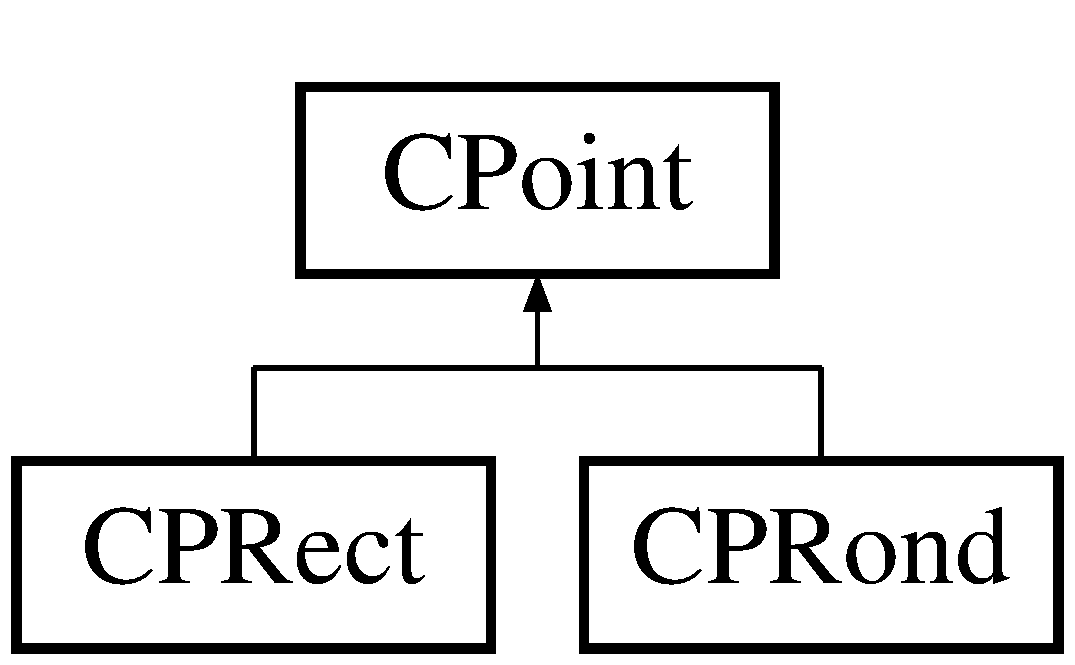
\includegraphics[height=2.000000cm]{class_c_point}
\end{center}
\end{figure}
\subsection*{Public Member Functions}
\begin{DoxyCompactItemize}
\item 
{\bfseries C\-Point} (int X, int Y, int Angle\-\_\-init, Q\-Color Color)\label{class_c_point_a8cb3a7054fee9f2b14e5934c5ae925f0}

\item 
int {\bfseries Get\-X} ()\label{class_c_point_aab5e444ca8b3e6e04abddf95c2eccdc5}

\item 
int {\bfseries Get\-Y} ()\label{class_c_point_aa4c063d7345446a61299f62a2f0edc51}

\item 
int {\bfseries Get\-Taille} ()\label{class_c_point_a58bdc2cf27e48c1f5aecd77f0727ba5e}

\item 
float {\bfseries Get\-Angle} ()\label{class_c_point_a973d12faf8432d9b712022d6d3a70f1c}

\item 
float {\bfseries Get\-Distance} ()\label{class_c_point_a5e932d56c5675df773fa2bdaac3eaae6}

\item 
bool {\bfseries Get\-Arriere} ()\label{class_c_point_a9ef10305782aa210d2d2906d69d10582}

\item 
int {\bfseries Get\-Delai} ()\label{class_c_point_a294cb016dfd6015a9911966cdeb61eef}

\item 
bool {\bfseries Get\-Servo\-Clap} ()\label{class_c_point_a77a908f05e2fcf3ced2ee246b9443662}

\item 
bool {\bfseries Get\-Servo\-Pince} ()\label{class_c_point_add4a0192e794997623b26ebc04a1f92a}

\item 
bool {\bfseries Get\-Capt\-Av} ()\label{class_c_point_a0981a37f9b3945989abe4fdf18ffa5d2}

\item 
bool {\bfseries Get\-Capt\-Ar} ()\label{class_c_point_aa0fb9e1e43e63c4ed5a4f4e111fe64d4}

\item 
int {\bfseries Get\-Angle\-Init} ()\label{class_c_point_aa454ce1065ae1fcebc9dad6eb6782811}

\item 
void {\bfseries Set\-Servo\-Clap} (int X)\label{class_c_point_ac7f0ffa1e3848a3bbda5cddab37e0f8a}

\item 
void {\bfseries Set\-Servo\-Pince} (bool X)\label{class_c_point_afe65922e719e51b08a91e2b22e668fea}

\item 
void {\bfseries Set\-Capt\-Av} (bool X)\label{class_c_point_a80ec358b9fc198e273952bcf945a241a}

\item 
void {\bfseries Set\-Capt\-Ar} (bool X)\label{class_c_point_a6c17d7d007140a80639728af3e97544c}

\item 
void {\bfseries Set\-Delai} (int time)\label{class_c_point_a238de9eca4a0955e5990a6f8e934918f}

\item 
void {\bfseries Set\-Angle\-Init} (int Angle)\label{class_c_point_a83b2d6f294cbbdb15f6fb733624ae539}

\item 
void {\bfseries Set\-Marche\-Arriere} (bool X)\label{class_c_point_a56337ba7727290fbd18cbcc0a3005da4}

\item 
void {\bfseries Set\-Coord\-Polaire} ({\bf C\-Point} $\ast$Point\-Av)\label{class_c_point_ae7e569157bfb3072136ab9ca7f06f34d}

\item 
virtual void {\bfseries Set\-Color} (Q\-Color C)=0\label{class_c_point_a6ac3592624147923e9b8975830b6630a}

\item 
virtual void {\bfseries Deplacement} (int X, int Y)=0\label{class_c_point_a41ae3701584ed0a1b24df5907aff3b1f}

\item 
virtual Q\-Graphics\-Item $\ast$ {\bfseries Get\-Type} ()=0\label{class_c_point_a77acca79d4f34791acc50e406aece01f}

\end{DoxyCompactItemize}
\subsection*{Protected Attributes}
\begin{DoxyCompactItemize}
\item 
int {\bfseries n\-X}\label{class_c_point_a56b43dbd9752a0a1a65810068c8e1b0e}

\item 
int {\bfseries n\-Y}\label{class_c_point_a9f7bb0cf46eb923de44bd076d6cba1dc}

\item 
float {\bfseries n\-Angle}\label{class_c_point_a2ed3dcfb4866c7310025e484944765f8}

\item 
int {\bfseries n\-Angle\-\_\-init}\label{class_c_point_a655c23394a707a26e15d39bd549678fc}

\item 
float {\bfseries n\-Distance}\label{class_c_point_a6297cd2c695cc6e55eff4b7ceab712a5}

\item 
int {\bfseries n\-Delai}\label{class_c_point_a4a1295bb2bbe0262745b28e804e339e4}

\item 
int {\bfseries Servo\-Clap}\label{class_c_point_a44375d1e2ba537374196a10d3ac54726}

\item 
bool {\bfseries Servo\-Pince}\label{class_c_point_ad09477e585b5c703ae78a8415a3875f9}

\item 
bool {\bfseries Capt\-Av}\label{class_c_point_a2104bc3202c15adc696878a7b730522c}

\item 
bool {\bfseries Capt\-Ar}\label{class_c_point_ac54cc9ceba8683ef772460af9557e13d}

\item 
bool {\bfseries b\-M\-Arriere}\label{class_c_point_a77fa347ab5df7055dda85ad160a7bac4}

\item 
float {\bfseries n\-Taille}\label{class_c_point_a180430062c8c3adbfceffd0e0b82f7b1}

\item 
Q\-Color $\ast$ {\bfseries p\-Couleur}\label{class_c_point_ab3333381fe54f81ac67257d006b22215}

\end{DoxyCompactItemize}


\subsection{Detailed Description}
Classe de base pour les différents type de points. 

\doxyref{C\-Point}{p.}{class_c_point} est une classe de base dont hérite les classes typées de points (\doxyref{C\-P\-Rect}{p.}{class_c_p_rect}, \doxyref{C\-P\-Rond}{p.}{class_c_p_rond}...) Contient toutes les variables correspondants à une étape. 

The documentation for this class was generated from the following files\-:\begin{DoxyCompactItemize}
\item 
Gestion\-\_\-\-Deplacements/cpoint.\-h\item 
Gestion\-\_\-\-Deplacements/cpoint.\-cpp\end{DoxyCompactItemize}

\section{C\-P\-Rect Class Reference}
\label{class_c_p_rect}\index{C\-P\-Rect@{C\-P\-Rect}}
Inheritance diagram for C\-P\-Rect\-:\begin{figure}[H]
\begin{center}
\leavevmode
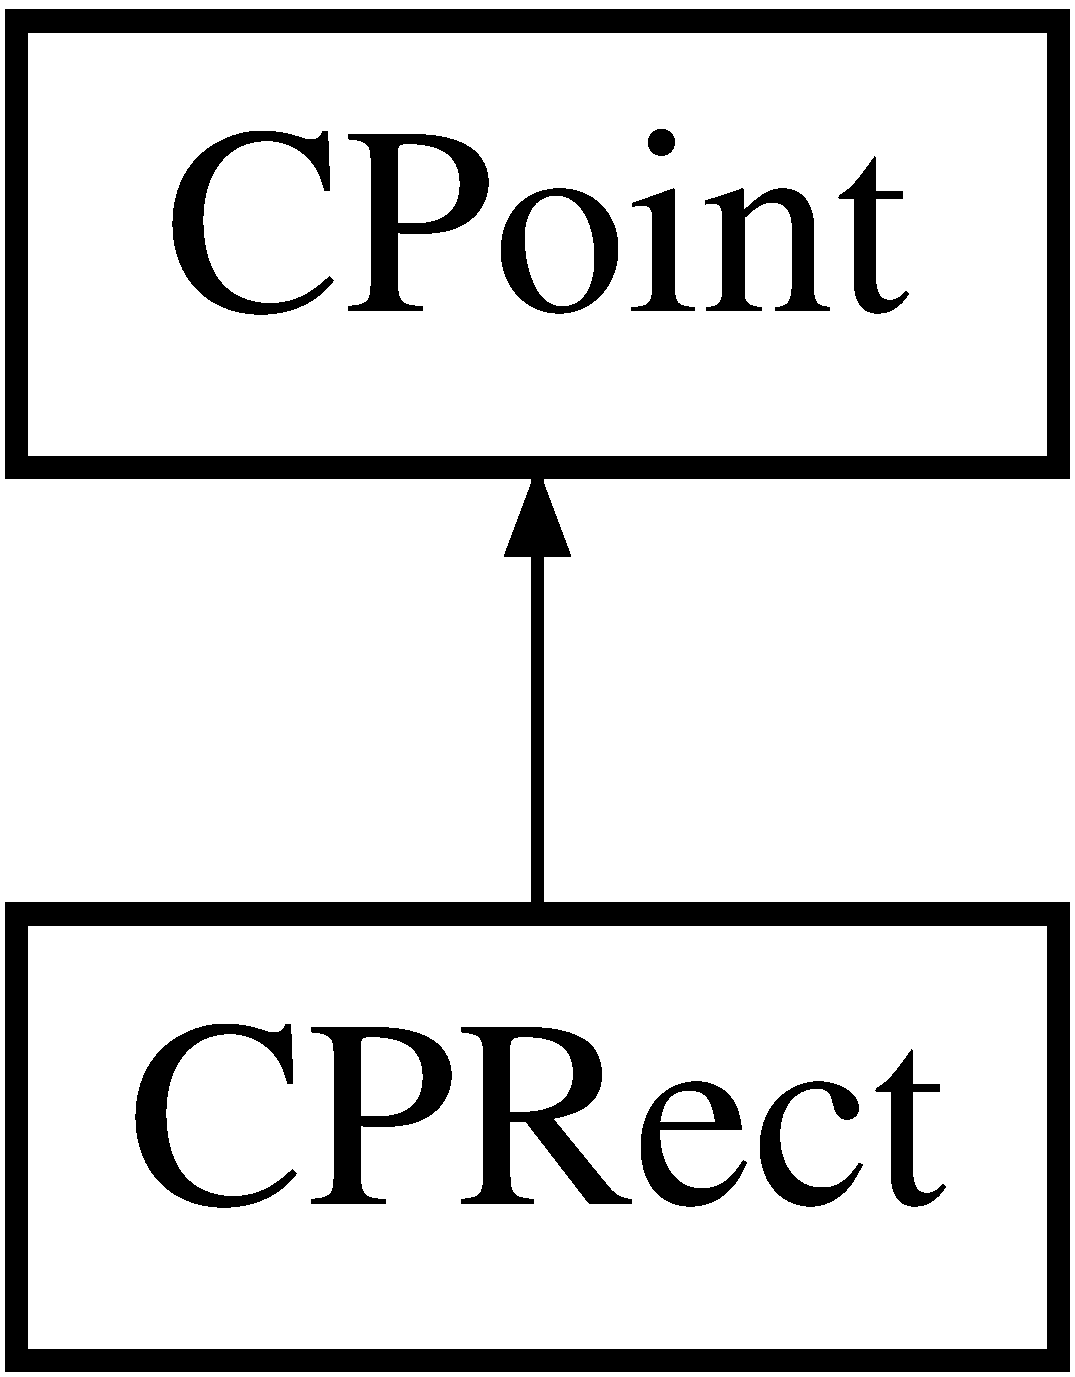
\includegraphics[height=2.000000cm]{class_c_p_rect}
\end{center}
\end{figure}
\subsection*{Public Member Functions}
\begin{DoxyCompactItemize}
\item 
{\bfseries C\-P\-Rect} (int X, int Y, int Angle, Q\-Color Color)\label{class_c_p_rect_a4fe959025240ac344d98dbfc01ed2ac0}

\item 
virtual void {\bfseries Deplacement} (int X, int Y)\label{class_c_p_rect_a72c14444cb2101761748a5b224834813}

\item 
virtual void {\bfseries Set\-Color} (Q\-Color C)\label{class_c_p_rect_a92a2b116e3b8ee6cb2b34a16a6f6cb3a}

\item 
virtual Q\-Graphics\-Item $\ast$ {\bfseries Get\-Type} ()\label{class_c_p_rect_abb8eb3cd2d131d549d02f9fdb87a47b1}

\end{DoxyCompactItemize}
\subsection*{Additional Inherited Members}


The documentation for this class was generated from the following files\-:\begin{DoxyCompactItemize}
\item 
Gestion\-\_\-\-Deplacements/cprect.\-h\item 
Gestion\-\_\-\-Deplacements/cprect.\-cpp\end{DoxyCompactItemize}

\section{C\-P\-Rond Class Reference}
\label{class_c_p_rond}\index{C\-P\-Rond@{C\-P\-Rond}}
Inheritance diagram for C\-P\-Rond\-:\begin{figure}[H]
\begin{center}
\leavevmode
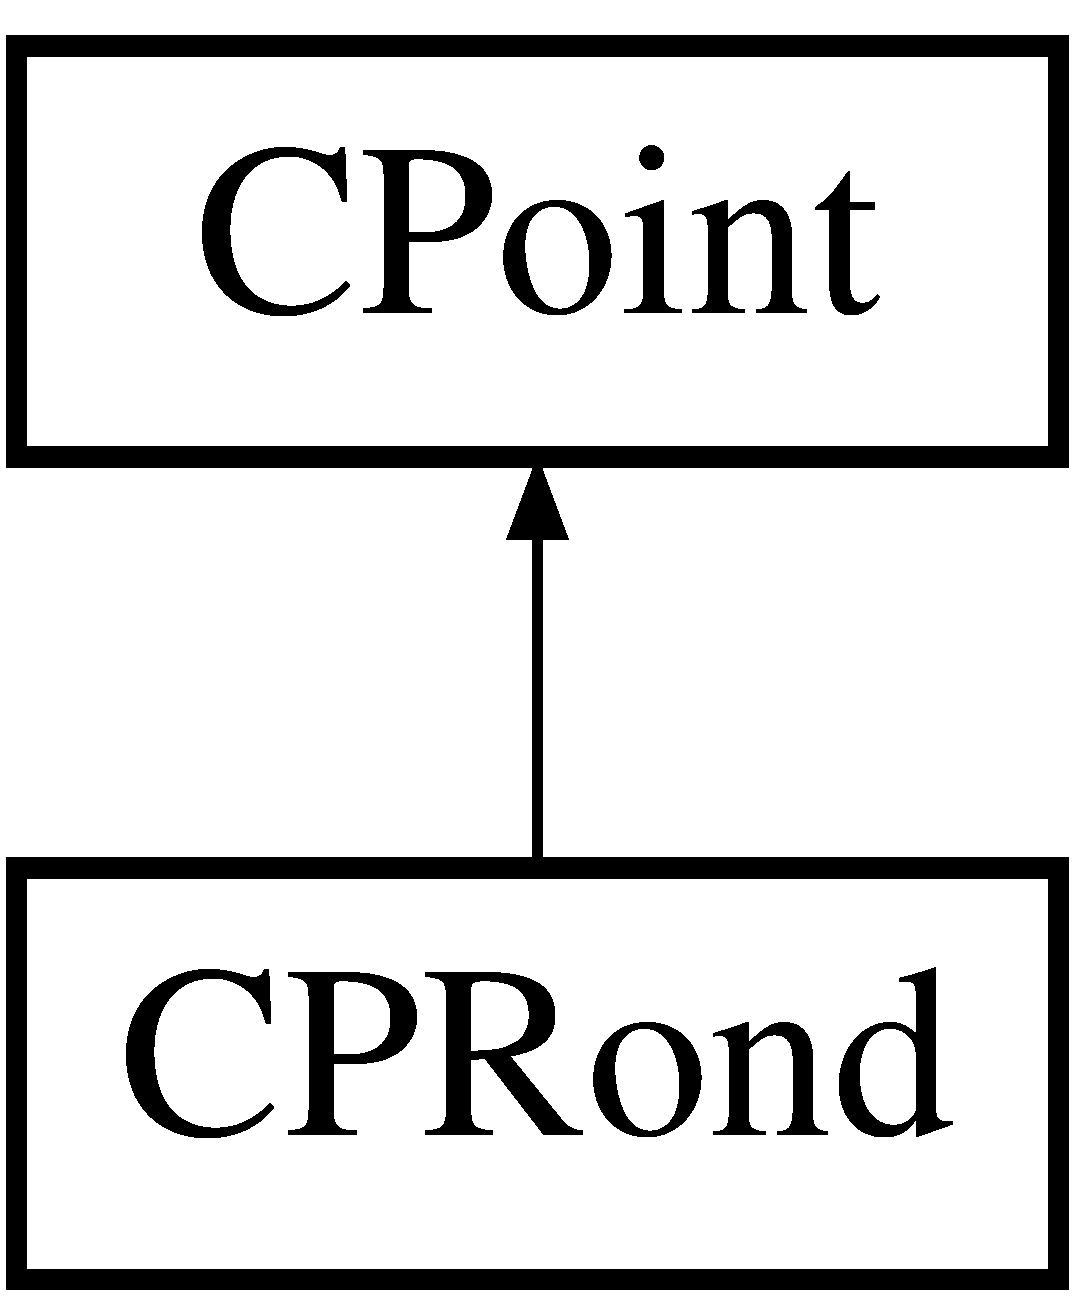
\includegraphics[height=2.000000cm]{class_c_p_rond}
\end{center}
\end{figure}
\subsection*{Public Member Functions}
\begin{DoxyCompactItemize}
\item 
{\bfseries C\-P\-Rond} (int X, int Y, int Angle, Q\-Color Color)\label{class_c_p_rond_a7057682137723d0f9b49f5851d880b9d}

\item 
virtual void {\bfseries Deplacement} (int X, int Y)\label{class_c_p_rond_ac514e0eb265ecf836a441adbb3408909}

\item 
virtual void {\bfseries Set\-Color} (Q\-Color C)\label{class_c_p_rond_a55d9d8cd91a5db50c10f74362cf9a47e}

\item 
virtual Q\-Graphics\-Item $\ast$ {\bfseries Get\-Type} ()\label{class_c_p_rond_add68fb9c3e149f4b5d1e0cf2e1b5211d}

\end{DoxyCompactItemize}
\subsection*{Additional Inherited Members}


The documentation for this class was generated from the following files\-:\begin{DoxyCompactItemize}
\item 
Gestion\-\_\-\-Deplacements/cprond.\-h\item 
Gestion\-\_\-\-Deplacements/cprond.\-cpp\end{DoxyCompactItemize}

\section{crobot Class Reference}
\label{classcrobot}\index{crobot@{crobot}}
\subsection*{Public Member Functions}
\begin{DoxyCompactItemize}
\item 
{\bfseries crobot} (int X, int Y, int Angle)\label{classcrobot_ab52a9bee95e1a9332c95362f7cbaabba}

\item 
Q\-Graphics\-Item $\ast$ {\bfseries Get\-Type} ()\label{classcrobot_a806d7430d838aa3ef1aca73ca90cdac3}

\item 
void {\bfseries Set\-Robot} (int X, int Y, int Angle)\label{classcrobot_ae49f9348cf518ce038a94b8be23c4403}

\end{DoxyCompactItemize}


The documentation for this class was generated from the following files\-:\begin{DoxyCompactItemize}
\item 
Gestion\-\_\-\-Deplacements/crobot.\-h\item 
Gestion\-\_\-\-Deplacements/crobot.\-cpp\end{DoxyCompactItemize}

\section{Ui\-:\-:Main\-Window Class Reference}
\label{class_ui_1_1_main_window}\index{Ui\-::\-Main\-Window@{Ui\-::\-Main\-Window}}
Inheritance diagram for Ui\-:\-:Main\-Window\-:\begin{figure}[H]
\begin{center}
\leavevmode
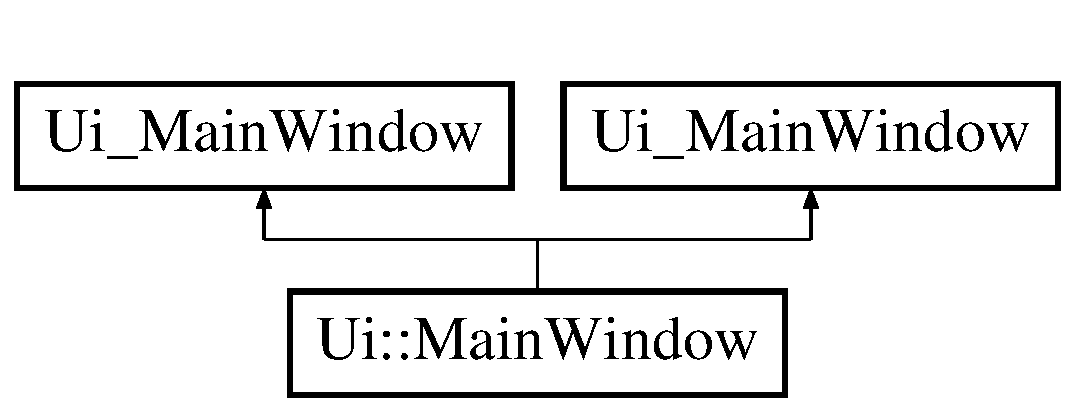
\includegraphics[height=2.000000cm]{class_ui_1_1_main_window}
\end{center}
\end{figure}
\subsection*{Additional Inherited Members}


The documentation for this class was generated from the following file\-:\begin{DoxyCompactItemize}
\item 
build-\/\-Gestion\-\_\-\-Deplacements-\/\-Desktop-\/\-Debug/ui\-\_\-mainwindow.\-h\end{DoxyCompactItemize}

\section{Main\-Window Class Reference}
\label{class_main_window}\index{Main\-Window@{Main\-Window}}
Inheritance diagram for Main\-Window\-:\begin{figure}[H]
\begin{center}
\leavevmode
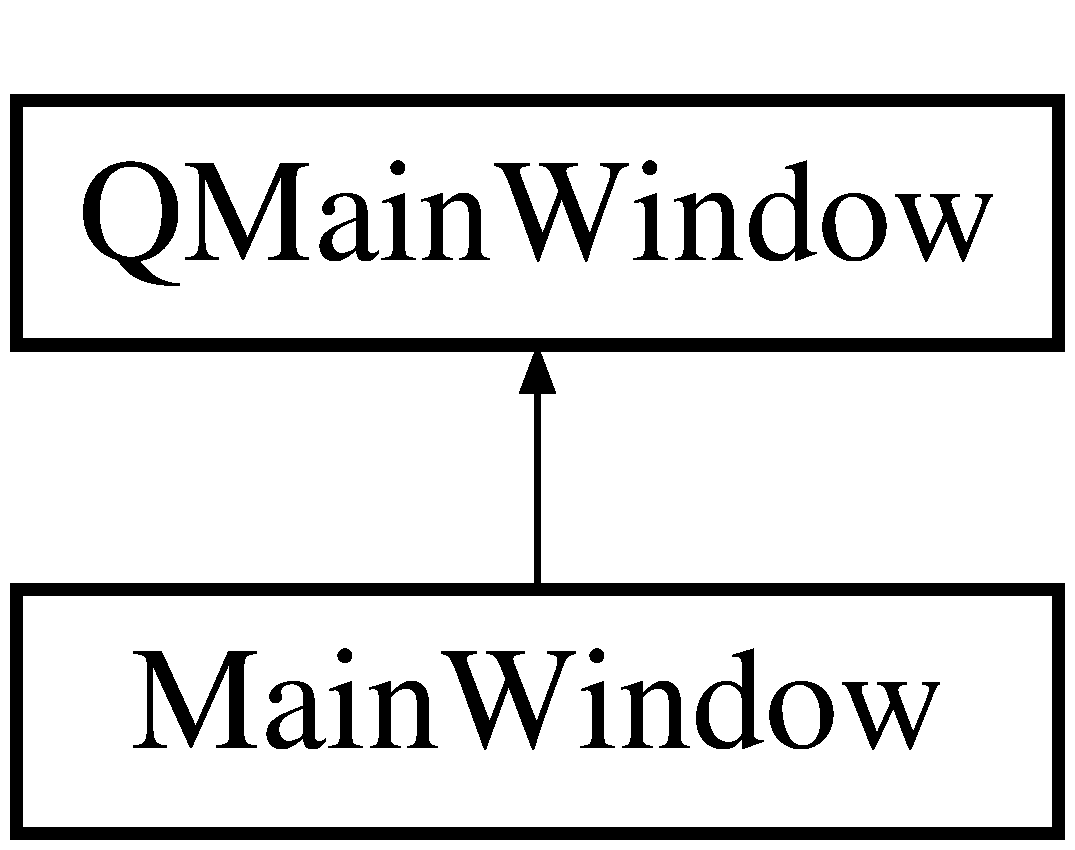
\includegraphics[height=2.000000cm]{class_main_window}
\end{center}
\end{figure}
\subsection*{Public Slots}
\begin{DoxyCompactItemize}
\item 
void {\bfseries Set\-Pos\-Souris\-Label} (int X, int Y)\label{class_main_window_afa42355eca5129bb79f26b363e18c596}

\item 
void {\bfseries Add\-Objet} (int X, int Y)\label{class_main_window_a63519d0197921f0b2865d9bfa877ff48}

\end{DoxyCompactItemize}
\subsection*{Public Member Functions}
\begin{DoxyCompactItemize}
\item 
{\bfseries Main\-Window} (Q\-Widget $\ast$parent=0)\label{class_main_window_a8b244be8b7b7db1b08de2a2acb9409db}

\item 
void {\bfseries Set\-Informations\-Etape} ()\label{class_main_window_a681fbce5a1d72f252749de90d1f8de7a}

\item 
void {\bfseries Set\-Liste\-Etapes} ()\label{class_main_window_a513b2ad8b54f69eb57e307a4cd436421}

\item 
void {\bfseries set\-X\-Y} (int X, int Y)\label{class_main_window_ad1ba6178941331412706c0579332dec9}

\end{DoxyCompactItemize}


The documentation for this class was generated from the following files\-:\begin{DoxyCompactItemize}
\item 
Gestion\-\_\-\-Deplacements/mainwindow.\-h\item 
Gestion\-\_\-\-Deplacements/mainwindow.\-cpp\end{DoxyCompactItemize}

\section{qt\-\_\-meta\-\_\-stringdata\-\_\-\-Main\-Window\-\_\-t Struct Reference}
\label{structqt__meta__stringdata___main_window__t}\index{qt\-\_\-meta\-\_\-stringdata\-\_\-\-Main\-Window\-\_\-t@{qt\-\_\-meta\-\_\-stringdata\-\_\-\-Main\-Window\-\_\-t}}
\subsection*{Public Attributes}
\begin{DoxyCompactItemize}
\item 
Q\-Byte\-Array\-Data {\bfseries data} [6]\label{structqt__meta__stringdata___main_window__t_af598c0b01c666753185a38017d12d5cc}

\item 
char {\bfseries stringdata} [44]\label{structqt__meta__stringdata___main_window__t_aa503b5aa1215c5044c71808a38a8c946}

\end{DoxyCompactItemize}


The documentation for this struct was generated from the following file\-:\begin{DoxyCompactItemize}
\item 
build-\/\-Gestion\-\_\-\-Deplacements-\/\-Desktop-\/\-Debug/moc\-\_\-mainwindow.\-cpp\end{DoxyCompactItemize}

\section{qt\-\_\-meta\-\_\-stringdata\-\_\-\-Q\-View\-Table\-\_\-t Struct Reference}
\label{structqt__meta__stringdata___q_view_table__t}\index{qt\-\_\-meta\-\_\-stringdata\-\_\-\-Q\-View\-Table\-\_\-t@{qt\-\_\-meta\-\_\-stringdata\-\_\-\-Q\-View\-Table\-\_\-t}}
\subsection*{Public Attributes}
\begin{DoxyCompactItemize}
\item 
Q\-Byte\-Array\-Data {\bfseries data} [4]\label{structqt__meta__stringdata___q_view_table__t_aacad6a9f84d6693be5938848d2cb1545}

\item 
char {\bfseries stringdata} [25]\label{structqt__meta__stringdata___q_view_table__t_a43b25bfc3e296e075ae0380ac079d230}

\end{DoxyCompactItemize}


The documentation for this struct was generated from the following file\-:\begin{DoxyCompactItemize}
\item 
build-\/\-Gestion\-\_\-\-Deplacements-\/\-Desktop-\/\-Debug/moc\-\_\-qviewtable.\-cpp\end{DoxyCompactItemize}

\section{Q\-View\-Table Class Reference}
\label{class_q_view_table}\index{Q\-View\-Table@{Q\-View\-Table}}
Inheritance diagram for Q\-View\-Table\-:\begin{figure}[H]
\begin{center}
\leavevmode
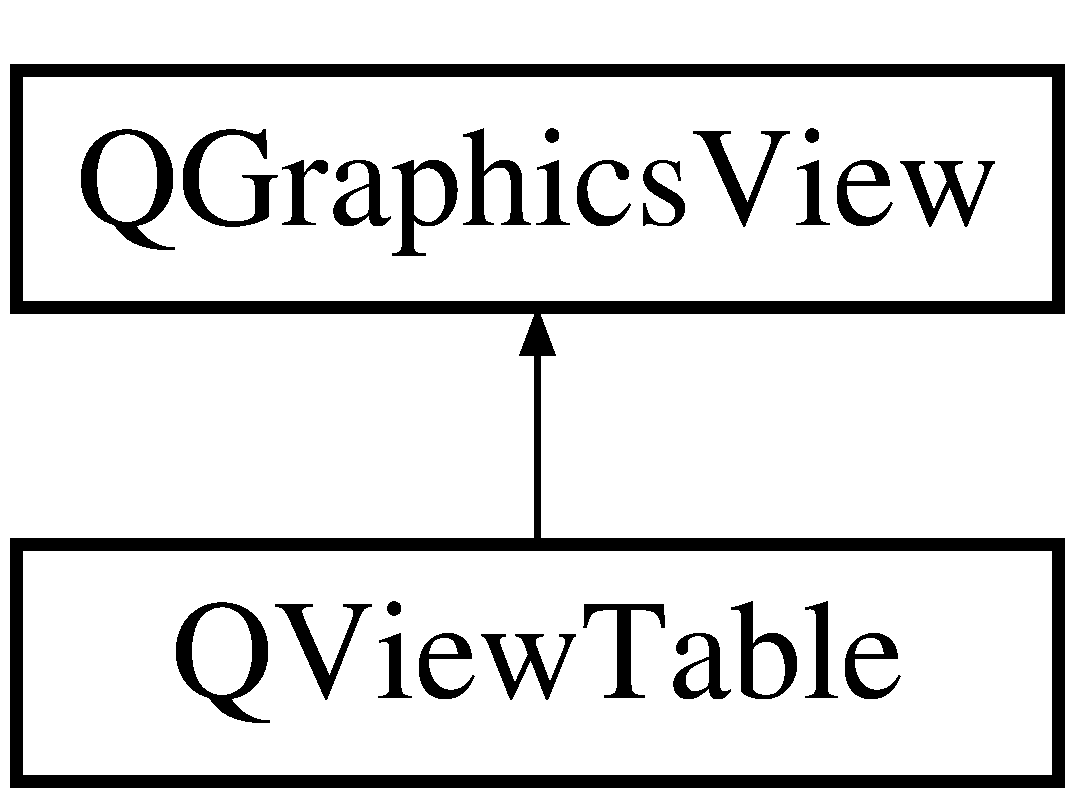
\includegraphics[height=2.000000cm]{class_q_view_table}
\end{center}
\end{figure}
\subsection*{Signals}
\begin{DoxyCompactItemize}
\item 
void {\bfseries Souris} (int, int)\label{class_q_view_table_aeed427b455f8922fb7809a9c9dcd583a}

\item 
void {\bfseries Clic} (int, int)\label{class_q_view_table_a789d3d7b06c4619f7df2b452d8f75a27}

\end{DoxyCompactItemize}
\subsection*{Public Member Functions}
\begin{DoxyCompactItemize}
\item 
{\bfseries Q\-View\-Table} (Q\-Widget $\ast$parent=0)\label{class_q_view_table_a7eb9f241410b3a84f22f86c7938cefa5}

\end{DoxyCompactItemize}
\subsection*{Protected Member Functions}
\begin{DoxyCompactItemize}
\item 
void {\bfseries mouse\-Move\-Event} (Q\-Mouse\-Event $\ast$event)\label{class_q_view_table_a5cfb236893278305f1e301deb263cceb}

\item 
void {\bfseries mouse\-Press\-Event} (Q\-Mouse\-Event $\ast$event)\label{class_q_view_table_a97a479e58095cecd7c929aece94024e3}

\end{DoxyCompactItemize}


The documentation for this class was generated from the following files\-:\begin{DoxyCompactItemize}
\item 
Gestion\-\_\-\-Deplacements/qviewtable.\-h\item 
build-\/\-Gestion\-\_\-\-Deplacements-\/\-Desktop-\/\-Debug/moc\-\_\-qviewtable.\-cpp\item 
Gestion\-\_\-\-Deplacements/qviewtable.\-cpp\end{DoxyCompactItemize}

\section{Ui\-\_\-\-Main\-Window Class Reference}
\label{class_ui___main_window}\index{Ui\-\_\-\-Main\-Window@{Ui\-\_\-\-Main\-Window}}
Inheritance diagram for Ui\-\_\-\-Main\-Window\-:\begin{figure}[H]
\begin{center}
\leavevmode
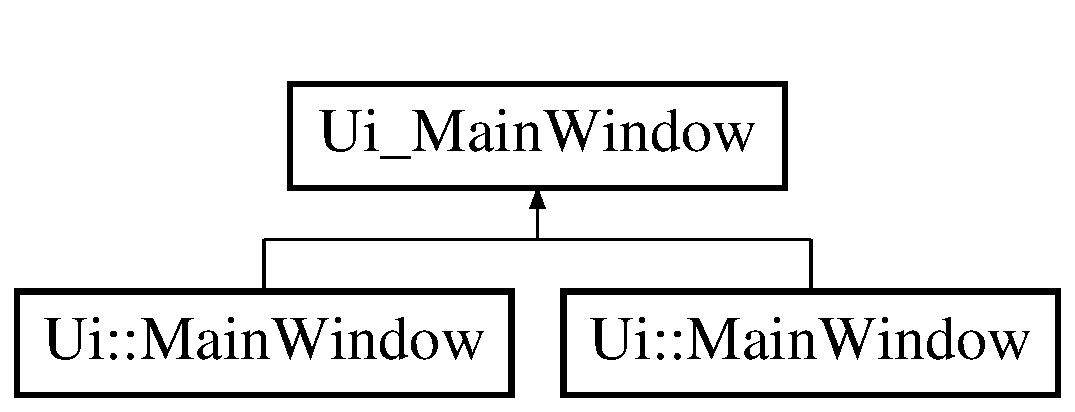
\includegraphics[height=2.000000cm]{class_ui___main_window}
\end{center}
\end{figure}
\subsection*{Public Member Functions}
\begin{DoxyCompactItemize}
\item 
void {\bfseries setup\-Ui} (Q\-Main\-Window $\ast${\bf Main\-Window})\label{class_ui___main_window_acf4a0872c4c77d8f43a2ec66ed849b58}

\item 
void {\bfseries retranslate\-Ui} (Q\-Main\-Window $\ast${\bf Main\-Window})\label{class_ui___main_window_a097dd160c3534a204904cb374412c618}

\item 
void {\bfseries setup\-Ui} (Q\-Main\-Window $\ast${\bf Main\-Window})\label{class_ui___main_window_acf4a0872c4c77d8f43a2ec66ed849b58}

\item 
void {\bfseries retranslate\-Ui} (Q\-Main\-Window $\ast${\bf Main\-Window})\label{class_ui___main_window_a097dd160c3534a204904cb374412c618}

\end{DoxyCompactItemize}
\subsection*{Public Attributes}
\begin{DoxyCompactItemize}
\item 
Q\-Widget $\ast$ {\bfseries central\-Widget}\label{class_ui___main_window_a6600dd3bdd3d55e535659e4a4096ea48}

\item 
Q\-H\-Box\-Layout $\ast$ {\bfseries horizontal\-Layout}\label{class_ui___main_window_ae7104d878681f568e492c5bd0f653157}

\item 
Q\-Frame $\ast$ {\bfseries frame}\label{class_ui___main_window_a0a6f09c1b54d40d3900cac8179e189bf}

\item 
Q\-V\-Box\-Layout $\ast$ {\bfseries vertical\-Layout\-\_\-2}\label{class_ui___main_window_afbe60c634b3214ee76ff9e1fa70c7801}

\item 
Q\-Spin\-Box $\ast$ {\bfseries spin\-Box}\label{class_ui___main_window_a0ecf336f5c740a4fe679d429781d0cb5}

\item 
Q\-Spacer\-Item $\ast$ {\bfseries vertical\-Spacer}\label{class_ui___main_window_a2c53f7f2e3106a4225d5be295e1315ae}

\item 
Q\-Push\-Button $\ast$ {\bfseries push\-Button\-\_\-4}\label{class_ui___main_window_a6db9cf2b9979472a16e8a7e79c1950bf}

\item 
Q\-Splitter $\ast$ {\bfseries splitter\-\_\-2}\label{class_ui___main_window_a59fddea9485f8346c7bb5d2126c547a0}

\item 
Q\-Splitter $\ast$ {\bfseries splitter}\label{class_ui___main_window_aa9aced3c49e5cad22d46b6fa7a3d5292}

\item 
{\bf Q\-View\-Table} $\ast$ {\bfseries Q\-Table}\label{class_ui___main_window_ac43fa751c51da69c2de7ec18be1bc3e0}

\item 
Q\-Frame $\ast$ {\bfseries frame\-\_\-3}\label{class_ui___main_window_a27f45274513176c15239705dfafc2ecb}

\item 
Q\-H\-Box\-Layout $\ast$ {\bfseries horizontal\-Layout\-\_\-2}\label{class_ui___main_window_a9ee21d2c2bc000e7a8ba931bacfc5a69}

\item 
Q\-Label $\ast$ {\bfseries q\-Pos\-Label}\label{class_ui___main_window_a5e8dba76e1cc0c8448e861882721000f}

\item 
Q\-Spacer\-Item $\ast$ {\bfseries horizontal\-Spacer}\label{class_ui___main_window_ae189b5a48fa6e6f4b6775f1f832afe9c}

\item 
Q\-Push\-Button $\ast$ {\bfseries Add\-Groupe}\label{class_ui___main_window_a3843edcf211085038db405ad945f3cbd}

\item 
Q\-Push\-Button $\ast$ {\bfseries Add\-Point}\label{class_ui___main_window_afcad753cc22e9a7dbc50397c713a6b14}

\item 
Q\-Push\-Button $\ast$ {\bfseries Supprimer}\label{class_ui___main_window_a8c5a711e2d5e2295b387f4181c000f8e}

\item 
Q\-Frame $\ast$ {\bfseries frame\-\_\-2}\label{class_ui___main_window_a0f39414677a19e516a363ce9e4207424}

\item 
Q\-V\-Box\-Layout $\ast$ {\bfseries vertical\-Layout}\label{class_ui___main_window_a649287f742c9a33b8444116dccb1b72b}

\item 
Q\-Splitter $\ast$ {\bfseries splitter\-\_\-3}\label{class_ui___main_window_a8a8b121fe909315159bc4d287c1c2488}

\item 
Q\-List\-Widget $\ast$ {\bfseries q\-List\-Etape}\label{class_ui___main_window_a595a0a6bc302e68cdac851c987153807}

\item 
Q\-Table\-Widget $\ast$ {\bfseries q\-Infos\-Etape}\label{class_ui___main_window_a5224b98a08efd2a04c917693ee64ef21}

\item 
Q\-Menu\-Bar $\ast$ {\bfseries menu\-Bar}\label{class_ui___main_window_a502a50d7dc22415f511336bdfb4318b9}

\item 
Q\-Tool\-Bar $\ast$ {\bfseries main\-Tool\-Bar}\label{class_ui___main_window_abca26371605d7c5235fab5188d4bdcf7}

\item 
Q\-Status\-Bar $\ast$ {\bfseries status\-Bar}\label{class_ui___main_window_afa919f3af6f2f526a70f1fa331f63724}

\item 
Q\-Graphics\-View $\ast$ {\bfseries Q\-Table}\label{class_ui___main_window_a4043b83f277a7f93920dd493ef154adf}

\item 
Q\-Push\-Button $\ast$ {\bfseries B\-Envoyer}\label{class_ui___main_window_a47c721626085d59a52f5e4d77bdd023c}

\item 
Q\-Table\-View $\ast$ {\bfseries table\-View\-\_\-2}\label{class_ui___main_window_a922f8b861682d7eb2dc7b723a2c3e6cc}

\end{DoxyCompactItemize}


The documentation for this class was generated from the following file\-:\begin{DoxyCompactItemize}
\item 
build-\/\-Gestion\-\_\-\-Deplacements-\/\-Desktop-\/\-Debug/ui\-\_\-mainwindow.\-h\end{DoxyCompactItemize}

%--- End generated contents ---

% Index
\newpage
\phantomsection
\addcontentsline{toc}{chapter}{Index}
\printindex

\end{document}
